% Simulated combined-paper manuscript: Q1 body segment only.
% Adapted from the workspace-provided HuaweiCup23 converted LaTeX template.
\documentclass[11pt,a4paper]{article}

\usepackage[a4paper,top=2.4cm,bottom=2.3cm,left=2.35cm,right=2.35cm,footskip=1.1cm]{geometry}
\usepackage{iftex}
\ifPDFTeX
  \usepackage[T1]{fontenc}
  \usepackage[utf8]{inputenc}
  \usepackage{newtxtext,newtxmath}
\else
  \usepackage{fontspec}
  \setmainfont{TeX Gyre Termes}
  \usepackage{unicode-math}
  \setmathfont{TeX Gyre Termes Math}
\fi
\usepackage{graphicx}
\usepackage{xcolor}
\usepackage{booktabs,tabularx,array,multirow}
\usepackage{enumitem}
\usepackage{microtype}
\usepackage{caption}
\usepackage{float}
\usepackage{fancyhdr}
\usepackage{titlesec}
\usepackage{tikz}
\usetikzlibrary{arrows.meta,positioning,shapes.geometric}
\usepackage[hidelinks]{hyperref}

\definecolor{Ink}{HTML}{18324A}
\definecolor{Accent}{HTML}{197C83}
\definecolor{Pale}{HTML}{EAF2F4}
\setlength{\parindent}{1.5em}
\setlength{\parskip}{0.15em}
\setlength{\emergencystretch}{2em}
\renewcommand{\baselinestretch}{1.08}
\setcounter{secnumdepth}{3}
\captionsetup{font=small,labelfont=bf,labelsep=period,skip=5pt}
\titleformat{\section}{\large\bfseries\color{Ink}}{\thesection}{0.65em}{}
\titleformat{\subsection}{\normalsize\bfseries\color{Ink}}{\thesubsection}{0.6em}{}
\titleformat{\subsubsection}{\normalsize\bfseries}{\thesubsubsection}{0.6em}{}
\titlespacing*{\section}{0pt}{1.2em}{0.45em}
\titlespacing*{\subsection}{0pt}{0.85em}{0.3em}
\titlespacing*{\subsubsection}{0pt}{0.6em}{0.2em}
\pagestyle{fancy}
\fancyhf{}
\fancyhead[L]{\small\color{Ink}Q1 \textbar{} UAV CARGO BATCHING}
\fancyhead[R]{\small\thepage}
\renewcommand{\headrulewidth}{0.35pt}
\renewcommand{\headrule}{\hbox to\headwidth{\color{Accent}\leaders\hrule height \headrulewidth\hfill}}
\setlength{\headheight}{22pt}
\renewcommand{\topfraction}{0.88}
\renewcommand{\bottomfraction}{0.72}
\renewcommand{\textfraction}{0.12}
\renewcommand{\floatpagefraction}{0.78}
\setcounter{topnumber}{3}
\setcounter{bottomnumber}{2}
\setcounter{totalnumber}{5}
\setlength{\textfloatsep}{10pt plus 2pt minus 2pt}
\setlength{\intextsep}{9pt plus 2pt minus 2pt}

\newcommand{\Ehor}{E^{\mathrm{hor}}}
\newcommand{\Eup}{E^{\mathrm{up}}}
\newcommand{\ND}{\operatorname{ND}}
\newcommand{\SOC}{\mathrm{SOC}}
\newcommand{\kWh}{\,\mathrm{kWh}}
\newcommand{\kg}{\,\mathrm{kg}}
\newcommand{\m}{\,\mathrm{m}}
\newcommand{\s}{\,\mathrm{s}}
\begin{document}
\begin{titlepage}
\thispagestyle{empty}
\centering
\vspace*{0.45cm}
\begin{tabular}{@{}c@{\hspace{0.35cm}}c@{\hspace{0.35cm}}c@{}}
  
\includegraphics[width=82pt,height=53pt,keepaspectratio]{figures/cpipc-logo.png} &
  
\includegraphics[width=64pt,height=62pt,keepaspectratio]{figures/contest-logo.png} &
  
\includegraphics[width=66pt,height=66pt,keepaspectratio]{figures/huawei-logo.png}\\
\end{tabular}\par
\vspace{1.05cm}
{\large\sffamily\bfseries\color{Ink}China Postgraduate Innovation \& Practice Competitions\par}
\vspace{0.35cm}
{\Large\sffamily\bfseries\color{Ink}The 23rd “Huawei Cup” China Post-Graduate\\[-0.05em]
Mathematical Contest in Modeling\par}
\vspace{0.25cm}
{\small\color{Accent}SIMULATION MANUSCRIPT — QUESTION 1 SECTION\par}
\vspace{0.7cm}
{\LARGE\bfseries\color{Ink}Modeling and Optimization for Emergency UAV Supply Transport\par}
\vspace{0.15cm}
{\large\color{Ink}Terrain-Constrained Cargo Batching and Multiobjective Planning\par}
\vspace{0.9cm}
\begin{minipage}{0.88\linewidth}
\centering
\renewcommand{\arraystretch}{1.35}
\begin{tabular}{@{}p{3.3cm}p{10cm}@{}}
\textbf{University} & \hrulefill\\ \hline
\textbf{Team Number} & \hrulefill\\ \hline
\multirow{3}{3.3cm}{\centering\textbf{Team Members}} & 1.\ \hrulefill\\
 & 2.\ \hrulefill\\
 & 3.\ \hrulefill\\ \hline
\end{tabular}
\end{minipage}
\vfill
{\small The supplied Huawei Cup template identity is retained for simulation fidelity.\\
This document contains only the Q1 body section of a larger combined manuscript.\par}
\vspace{0.3cm}
{\small English single-column working draft \textbar{} 25 September 2026\par}
\end{titlepage}

\pagenumbering{arabic}

\section{Question 1: Terrain-Constrained UAV Cargo Batching}
\subsection{Problem and data}
\subsubsection{Mathematical restatement}
Let $S=\{1,\ldots,15\}$ be the service areas, $C_s$ the cargo boxes assigned to area $s$, and $G=\{A,B,C\}$ the aircraft models. A sortie chooses one area $s$, one aircraft model $g$, and one nonempty subset $B\subseteq C_s$. It flies depot $O01\to s$, transfers all boxes in $B$, and returns $s\to O01$ without cargo. Every box is delivered once; boxes are not split or mixed across service areas. The objectives are to minimize the total number of sorties $N$, total modeled energy $E$, and total cumulative operating time $T$.

The dataset contains 80 boxes with a combined mass of 758 kg and a combined volume of 2.011 m$^3$. Each area has between 3 and 15 boxes. The aircraft loading limits in Table~\ref{tab:aircraft} are hard constraints; the continuous payload calculation is energy- and range-based and does not impose volume, while each actual box subset must satisfy both mass and volume limits.

\begin{table}[H]
\centering
\caption{Nominal aircraft loading limits used in Q1.}
\label{tab:aircraft}
\begin{tabular}{lrr}
\toprule
Aircraft model & Maximum cargo mass (kg) & Loading volume (m$^3$)\\
\midrule
A & 25 & 0.060\\
B & 30 & 0.073\\
C & 80 & 0.250\\
\bottomrule
\end{tabular}
\end{table}

Figures~\ref{fig:q1-mass-profile}--\ref{fig:q1-area-demand} summarize the original input distribution without fitting statistical models. Cargo masses are discrete, so Fig.~\ref{fig:q1-mass-profile} reports frequencies rather than a continuous density. Figure~\ref{fig:q1-mass-volume} displays every supplied mass--volume pair without jitter, and Fig.~\ref{fig:q1-area-demand} shows all 15 area counts.

\begin{figure}[H]\centering
\includegraphics[width=0.55\linewidth,height=0.68\textheight,keepaspectratio]{figs/q1_fig01_mass_profile.pdf}\caption{Frequency of the 80 supplied cargo-box masses (kg). Exact counts are shown; no continuous density is fitted.}\label{fig:q1-mass-profile}\end{figure}
\begin{figure}[H]\centering
\includegraphics[width=0.55\linewidth,height=0.68\textheight,keepaspectratio]{figs/q1_fig02_mass_volume.pdf}\caption{Mass--volume pairs for all 80 boxes by cargo class. Coordinates are unjittered source values.}\label{fig:q1-mass-volume}\end{figure}
\begin{figure}[H]\centering
\includegraphics[width=0.55\linewidth,height=0.68\textheight,keepaspectratio]{figs/q1_fig03_area_demand.pdf}\caption{Exact number of cargo boxes assigned to each service area; all 15 areas are shown.}\label{fig:q1-area-demand}\end{figure}

\subsubsection{Input processing and scope}
The workbooks are read by named columns and sheets; the service-area demand summary is not treated as additional cargo. Cargo IDs are checked for uniqueness, every area must be represented, and positive finite mass and volume are required. Coordinates are projected to a local metric system before distances are calculated. For each depot--area segment, the route is sampled against intersected DEM cells; the maximum terrain elevation defines the cruise altitude. A route outside the valid DEM domain or intersecting NoData is not silently assigned a height: the affected candidate is treated as unverifiable and excluded pending data correction.

\subsection{Physical feasibility model}
\subsubsection{Terrain, range, and flight time}
For a directed leg $i\to j$, let $d_{ij}$ denote the projected horizontal distance and $z^{\max}_{ij}$ the maximum DEM elevation along the straight horizontal route. The specified cruise altitude and climb/descent increments are
\begin{align}
z^{\mathrm{cr}}_{ij}&=z^{\max}_{ij}+50\m,\\
h^+_{ij}&=\max\{0,z^{\mathrm{cr}}_{ij}-z_i^{\mathrm{op}}\},\qquad
h^-_{ij}=\max\{0,z^{\mathrm{cr}}_{ij}-z_j^{\mathrm{op}}\},
\end{align}
where the depot operates at its supplied elevation and a service-area aircraft operates 30 m above its supplied elevation. For aircraft model $g$, the payload-dependent range $L_g(q)$ and leg time $t_{gij}$ follow the supplied range and speed relationships:
\begin{align}
L_g(q)&=L_g^0-(L_g^0-L_g^F)\left(\frac{q}{Q_g}\right)^{3/2},\quad 0\le q\le Q_g,\label{eq:range}\\
t_{gij}&=\frac{h^+_{ij}}{v_g^\uparrow}+\frac{d_{ij}}{v_g^c}+\frac{h^-_{ij}}{v_g^\downarrow}.\label{eq:time}
\end{align}
Here $Q_g$ is rated payload, $L_g^0,L_g^F$ are unloaded and fully loaded ranges, and $v_g^\uparrow,v_g^c,v_g^\downarrow$ are climb, cruise, and descent speeds.

\subsubsection{Conditional energy convention}
The task describes energy as horizontal plus ascent energy but does not provide explicit component equations. We therefore define, and do not attribute to the task as a uniquely prescribed law, the baseline convention
\begin{align}
\Ehor_{gij}(q)&=E_g^{\mathrm{use}}\frac{d_{ij}}{L_g(q)},\\
\Eup_{gij}(q)&=\frac{(M_g+q)g h^+_{ij}}{3.6\times10^6\eta_g^\uparrow},\\
E_{gij}(q)&=\Ehor_{gij}(q)+\Eup_{gij}(q),
\label{eq:energy}
\end{align}
where $E_g^{\mathrm{use}}$ is usable battery energy in kWh, $M_g$ is empty aircraft mass including the battery in kg, $g=9.81\ \mathrm{m\,s^{-2}}$, $h^+$ is in metres, and $\eta_g^\uparrow$ is climb efficiency. The first term allocates usable energy in proportion to distance divided by payload-adjusted range; the second converts $mgh/\eta$ from joules to kWh. Descent has no separate energy term under this convention. Its adequacy depends on standard range representing horizontal cruise and usable battery energy reflecting unavailable reserve energy as recorded in the input.

For a cargo subset $B$ with total mass $m(B)$, the outbound leg carries $m(B)$ and the return leg is empty. Thus
\begin{equation}
E_{gsB}=E_{g,O01,s}(m(B))+E_{g,s,O01}(0),\qquad
\SOC^{\mathrm{return}}_{gsB}=1-\frac{E_{gsB}}{E_g^{\mathrm{use}}}\ge \rho_g.
\label{eq:roundtrip}
\end{equation}
Range is checked separately by $d_{O01,s}/L_g(m(B))+d_{s,O01}/L_g(0)\le1$. This prevents the common but incorrect substitution of a loaded round trip for a loaded outbound plus empty return. The continuous safe payload is
\begin{equation}
q^{\max}_{gs}=\max\{q\in[0,Q_g]: E_{g,O01,s}(q)+E_{g,s,O01}(0)\le(1-\rho_g)E_g^{\mathrm{use}}\}.
\label{eq:qmax}
\end{equation}
If even an empty round trip violates the reserve, the pair $(g,s)$ is reported unreachable rather than assigned a zero-kilogram capacity. Actual subsets are additionally subject to $m(B)\le Q_g$ and $v(B)\le V_g$; volume is intentionally absent from Eq.~\eqref{eq:qmax}.

The reserve baseline is $\rho=0.20$. To expose dependence on the unspecified energy split, we also scale horizontal and ascent components by $\alpha,\beta\in\{0.9,1.0,1.1\}$ and repeat the complete solve for reserves $\rho\in\{0.20,0.30,0.40\}$. These multipliers are diagnostic perturbations, not empirically estimated uncertainty bounds or official parameter ranges. Accordingly, all reported capacities, feasibility conclusions, Pareto fronts, and energy values are conditional on Eqs.~\eqref{eq:energy} and the stated scenario grid.

\subsection{Discrete batching and objectives}
\subsubsection{Feasible candidate set}
For each area, every nonempty cargo subset is paired with each of the three aircraft types. Candidate $b=(s,g,B)$ is retained only if
\begin{equation}
m(B)\le Q_g,\qquad v(B)\le V_g,\qquad
E_{gsB}\le(1-\rho_g)E_g^{\mathrm{use}},\qquad
\frac{d_{O01,s}}{L_g(m(B))}+\frac{d_{s,O01}}{L_g(0)}\le1.
\label{eq:candidate}
\end{equation}
No candidate cap is imposed. Since $|C_s|\le15$, area-wise exhaustive enumeration is bounded by $3(2^{|C_s|}-1)$ model--subset pairs before physical pruning.

Let $x_b\in\{0,1\}$ indicate selection of candidate $b$, and $C_b$ its box set. The exact set-partitioning requirements are
\begin{equation}
\sum_{b:c\in C_b}x_b=1\quad(\forall c\in C),\qquad x_b\in\{0,1\}.
\label{eq:partition}
\end{equation}
This equality enforces both complete delivery and no duplicate delivery. For each sortie, the modeled operating time includes round-trip flight, baseline handover, per-box handover, preflight preparation, and per-box loading:
\begin{equation}
T_b=t_{g,O01,s}+t_{g,s,O01}+t_g^{\mathrm{prep}}+|C_b|t_g^{\mathrm{load}}+t_g^{\mathrm{hand,base}}+|C_b|t_g^{\mathrm{hand,box}}.
\label{eq:batchtime}
\end{equation}
We minimize the vector
\begin{equation}
\min\;(F_N,F_E,F_T)=\left(\sum_bx_b,\ \sum_bE_bx_b,\ \sum_bT_bx_b\right).
\label{eq:objectives}
\end{equation}
$F_T$ is cumulative operating time summed over sorties. Q1 assigns no individual airframes and models no parallel execution, so it is not a fleet makespan and should not be interpreted as elapsed wall-clock completion time.

\subsubsection{Exact subset dynamic programming}
For area $s$ and local cargo subset $U\subseteq C_s$, let $P_s(U)$ contain the nondominated triples $(N,E,T)$ and their realizing partitions. Set $P_s(\varnothing)=\{(0,0,0)\}$. For nonempty $U$, let $i(U)$ be its lowest-indexed box and consider only feasible batches containing it:
\begin{equation}
P_s(U)=\ND\left\{(1,E_b,T_b)+p:\ b\in\mathcal B_s,\ C_b\subseteq U,\ i(U)\in C_b,\ p\in P_s(U\setminus C_b)\right\}.
\label{eq:dp}
\end{equation}
Anchoring every transition at the lowest uncovered box generates each partition once. At a fixed coverage mask, a dominated partial objective vector can be discarded: any continuation adds the same feasible future batch vectors, and therefore cannot make the dominated vector nondominated. After each area's full set has been solved, area fronts are combined by Minkowski addition and Pareto pruning:
\begin{equation}
\mathcal P=\ND\left(P_1(C_1)\oplus P_2(C_2)\oplus\cdots\oplus P_{15}(C_{15})\right).
\label{eq:merge}
\end{equation}
The decomposition is valid because Q1 has no shared aircraft, battery, charging, or inter-area timing constraints. Exactness is with respect to the fully enumerated candidates and the recorded floating-point comparison tolerances. This recurrence follows the established use of dynamic programming for discrete multicriteria optimization, while the area-wise state decomposition is tailored to this instance \cite{carraway1990,ehrgott2000}.

The workflow in Fig.~\ref{fig:q1-workflow} separates physical feasibility, exact combinatorial optimization, and result auditing. The epsilon grid is a downstream audit/read-out over the completed front: it does not generate the front and does not invoke a MILP.

\begin{figure}[H]
\centering
\begin{tikzpicture}[
  node distance=0.48cm,
  processbox/.style={draw=Accent,rounded corners=2pt,fill=Pale,align=center,text width=0.78\linewidth,minimum height=0.62cm,font=\small},
  arr/.style={-{Stealth[length=2mm]},thick,color=Accent}]
  \node[processbox] (data) {Cargo, aircraft, depot/service-area coordinates, and 30-m DEM};
  \node[processbox,below=of data] (physics) {Terrain profile, loaded-outbound / empty-return range and conditional energy};
  \node[processbox,below=of physics] (enum) {Exhaustive area-wise subset--aircraft enumeration; mass, volume, range, and reserve checks};
  \node[processbox,below=of enum] (dp) {Exact subset DP within each area; remove only dominated states at identical coverage};
  \node[processbox,below=of dp] (merge) {Minkowski merge of 15 area fronts and global nondominance pruning};
  \node[processbox,below=of merge] (report) {Epsilon-grid audit records; scenario feasibility, Pareto endpoints, and representative plan};
  \draw[arr] (data)--(physics); \draw[arr] (physics)--(enum); \draw[arr] (enum)--(dp); \draw[arr] (dp)--(merge);
  \draw[arr] (merge)--(report);
\end{tikzpicture}
\caption{Q1 solution workflow. Epsilon records audit the exact front; they are not separate MILP solves.}
\label{fig:q1-workflow}
\end{figure}

\subsubsection{Pareto interpretation and representative plan}
A solution dominates another if it is no worse in all three objectives and strictly better in at least one. We retain the complete nondominated set rather than imposing an arbitrary scalar trade-off during optimization. For descriptive comparison, each objective's ideal value $L_j$ and nadir value $U_j$ are computed from the complete front. The representative plan minimizes its equal-weight Euclidean distance to the normalized ideal:
\begin{equation}
\widehat F_j(x)=\begin{cases}(F_j(x)-L_j)/(U_j-L_j),&U_j>L_j,\\0,&U_j=L_j,\end{cases}\qquad
x^{\mathrm{rep}}=\arg\min_{x\in\mathcal P}\sqrt{\sum_{j\in\{N,E,T\}}\widehat F_j(x)^2}.
\label{eq:representative}
\end{equation}
Ties within numerical tolerance are resolved by sortie count, energy, cumulative time, and then canonical plan ID. This is a declared decision rule for a representative, not a claim that the selected plan is universally optimal under every stakeholder preference.

\subsection{Computational procedure and verification}
The implementation first computes area route geometries and aircraft physics, then enumerates feasible subsets and applies the local Pareto DP. Global front merging is followed by an epsilon-grid audit, representative-plan selection, and independent reconstruction of each reported partition. The code uses Python 3.12.14 and SciPy 1.18.1; the exact front is generated by the project implementation in \texttt{src/models/q1\_full.py}, with route physics in \texttt{src/models/q1\_physics.py}. No machine-learning surrogate or stochastic search is used to certify optimality.

In a repository checkout with \texttt{uv}, reproduce the full experiment and exports with:
\begin{quote}\small\ttfamily\raggedright
uv run --locked python -m src.experiments.q1\_full --scenario all --max-scenarios 27 --resume\par
uv run --locked python -m src.experiments.q1\_full\_report\par
uv run --locked python -m src.visualization.q1\_full\_figures
\end{quote}

The validation record reports 27/27 scenario outcomes resolved: 18 feasible scenarios have complete exact fronts and nine are proven infeasible. Candidate and DP results are fingerprinted against the source workbooks, DEM, model code, and lockfile. Validation checks cargo uniqueness, per-batch mass and volume, loaded outbound versus empty return, range, energy reserve, time-component reconciliation, and objective totals. The independent model review passed with conditions: the energy convention in Eqs.~\eqref{eq:energy} must be disclosed. The original epsilon records (10,184 across the experiment) are grid status records, not 10,184 MILP solves; epsilon enumeration is an audit of already-computed fronts.

Figure~\ref{fig:q1-candidate-reduction} summarizes how exhaustive raw model--subset combinations are reduced by physical checks and same-subset dominance pruning. Figure~\ref{fig:q1-epsilon-audit} shows the exact audit-record status by primary objective, pooled only over globally feasible scenarios.

\begin{figure}[H]\centering
\includegraphics[width=0.55\linewidth,height=0.68\textheight,keepaspectratio]{figs/q1_fig04_candidate_reduction.pdf}\caption{Candidate counts at each enumeration stage across 27 scenarios. The line is the median and the band is the empirical interquartile range, not a confidence interval; the vertical axis is logarithmic.}\label{fig:q1-candidate-reduction}\end{figure}
\begin{figure}[H]\centering
\includegraphics[width=0.55\linewidth,height=0.68\textheight,keepaspectratio]{figs/q1_fig05_epsilon_certification.pdf}\caption{Feasible and infeasible epsilon-grid records by primary objective, pooled over the 18 globally feasible scenarios. These are exact front-based certificates, not sampled data or MILP execution counts.}\label{fig:q1-epsilon-audit}\end{figure}
\subsection{Results and discussion}
\subsubsection{Safe payload and baseline feasibility}
For the baseline $(\rho,\alpha,\beta)=(0.20,1,1)$, the exported capacity table contains 45 aircraft--area pairs. Fifteen A-model pairs are bounded by the 25-kg rated payload, 14 B pairs by 30 kg, and 10 C pairs by 80 kg; the remaining six are energy-bound at lower values. This distinction is important: the capacity envelope is not uniform across all areas even though the nominal limits bind for most pairs. Figure~\ref{fig:q1-capacity} presents each computed value; these are energy/range safe payloads and do not replace subset-level volume screening.

\begin{figure}[H]\centering
\includegraphics[width=0.98\linewidth,height=0.45\textheight,keepaspectratio]{figs/q1_fig07_capacity_envelope.pdf}\caption{Maximum safe payload (kg) for each aircraft--area pair at the baseline parameter setting. Color and cell annotations encode the same computed value; an em dash marks an unreachable aircraft--area pairing.}\label{fig:q1-capacity}\end{figure}

Across the 27 modeled scenarios, feasibility declines as the return reserve rises: all nine $(\alpha,\beta)$ combinations are feasible at $\rho=0.20$, six are feasible at $\rho=0.30$, and three at $\rho=0.40$. Figure~\ref{fig:q1-front-cardinality} reports the exact front size in each scenario; an X marks a proven-infeasible full partition, not a zero-cardinality feasible front. The infeasible cases arise in the complete partitioning model; no hard constraint is relaxed to force a plan, and feasibility is therefore scenario-specific rather than a timeout artifact.
\begin{figure}[H]\centering
\includegraphics[width=0.98\linewidth,height=0.45\textheight,keepaspectratio]{figs/q1_fig06_frontier_cardinality.pdf}\caption{Cardinality of the complete exact nondominated objective set for each reserve and energy-multiplier combination. X marks a proven-infeasible scenario.}\label{fig:q1-front-cardinality}\end{figure}

\subsubsection{Exact baseline trade-off}
The baseline front contains exactly two distinct objective vectors (Table~\ref{tab:baseline}). The 18-sortie plan is both the minimum-sortie and minimum-cumulative-time endpoint in this two-point front; the 19-sortie plan is the minimum-energy endpoint. The representative rule in Eq.~\eqref{eq:representative} selects the 18-sortie point. It uses 0.09736 kWh (about 0.165\%) more than the energy-minimizing endpoint, while saving one sortie and 1,663.973 s of cumulative operating time. Figure~\ref{fig:q1-pareto} plots the pairwise projections; the points are deterministic nondominated plans, not repeated trials.

\begin{table}[H]
\centering
\caption{Complete baseline Pareto front and selected representative.}
\label{tab:baseline}
\begin{tabularx}{\linewidth}{@{}lrrr>{\raggedright\arraybackslash}X@{}}
\toprule
Plan & Sorties & Energy (kWh) & Cumulative time (s) & Interpretation\\
\midrule
Representative & 18 & 59.131669 & 32,776.093 & Equal-weight normalized ideal-distance rule; fewer sorties\\
Minimum-energy endpoint & 19 & 59.034314 & 34,440.065 & Lowest energy on the complete front\\
\bottomrule
\end{tabularx}
\end{table}

\begin{figure}[H]\centering
\includegraphics[width=0.98\linewidth,height=0.50\textheight,keepaspectratio]{figs/q1_fig08_baseline_pareto.pdf}\caption{Pairwise projections of both distinct objective vectors on the complete baseline Pareto front. The star identifies the selected representative and the diamond the minimum-energy endpoint; no statistical error bars apply.}\label{fig:q1-pareto}\end{figure}

The representative plan has 18 sorties: nine use model B and nine use model C; model A is not selected in this baseline representative. Figure~\ref{fig:q1-manifest} shows the per-sortie mass composition by cargo class. Its source reconciliation confirms that the selected batches contain all 80 distinct cargo IDs exactly once; each bar is a planned batch, not an observed flight. In the exported plan, every B sortie carries 25 kg and these nine batches contain 27 boxes; the C sorties carry 45--78 kg (mean 59.22 kg) and contain the remaining 53 boxes. This split describes the selected Pareto representative only, rather than a general dispatch rule.

\begin{figure}[H]\centering
\includegraphics[width=0.98\linewidth,height=0.58\textheight,keepaspectratio]{figs/q1_fig09_sortie_manifest.pdf}\caption{Cargo-class mass composition (kg) for each of the 18 representative sorties, split by aircraft model. Stacks sum to each sortie's payload; all 80 source cargo IDs occur exactly once.}\label{fig:q1-manifest}\end{figure}

\subsubsection{Reserve and energy sensitivity}
Each point on the sensitivity grid triggers a complete re-enumeration and re-optimization; it does not reuse the baseline partition. Figure~\ref{fig:q1-sensitivity} reports representative total-energy change relative to the baseline representative when a feasible representative exists. The gray infeasible cells are not assigned artificial energy values. The pattern should be interpreted jointly with feasibility: a reserve increase can eliminate the full assignment rather than merely increase energy. The $\alpha$ and $\beta$ grid is a structured model-diagnostic experiment, not a probability distribution, so we report no confidence interval or probabilistic robustness claim.

\begin{figure}[H]\centering
\includegraphics[width=0.98\linewidth,height=0.45\textheight,keepaspectratio]{figs/q1_fig10_energy_sensitivity.pdf}\caption{Change in selected representative total energy (kWh) from baseline over the reserve and energy-multiplier grid. Each feasible cell is fully re-solved; X denotes a proven-infeasible scenario.}\label{fig:q1-sensitivity}\end{figure}

\subsubsection{Limitations}
The largest limitation is structural: the explicit energy components are not supplied by the task, and the baseline equations are an interpretable modeling convention rather than a uniquely verified aircraft energy law. The multiplier experiment tests local sensitivity to that choice but cannot substitute for manufacturer flight logs or a calibrated propulsion model. Terrain is represented by the maximum intersected DEM elevation on a straight horizontal route; wind, weather, payload-dependent climb efficiency, turning, landing-site constraints, battery aging, and stochastic failure are not modeled. Finally, Q1 sums sortie operating times without assigning vehicles or scheduling concurrency. Consequently, its time objective cannot be read as response time or fleet makespan. These issues motivate richer Q2/Q3 scheduling, but those problems are outside the present paper's solved scope.

\phantomsection
\begin{thebibliography}{9}
\bibitem{carraway1990}
R. L. Carraway, T. L. Morin, and H. Moskowitz, ``Generalized dynamic programming for multicriteria optimization,'' \textit{European Journal of Operational Research}, vol. 44, no. 1, pp. 95--104, 1990, doi: 10.1016/0377-2217(90)90318-6.

\bibitem{ehrgott2000}
M. Ehrgott and X. Gandibleux, ``A survey and annotated bibliography of multiobjective combinatorial optimization,'' \textit{OR Spectrum}, vol. 22, pp. 425--460, 2000, doi: 10.1007/s002910000046.
\end{thebibliography}

\end{document}
